\section{Khám phá và trực quan hóa dữ liệu (Exploratory Data Analysis)}

\subsection{Tiền xử lý và kết xuất dữ liệu (Data Preparation \& Export)}
Quy trình tiền xử lý được thực hiện nhằm đảm bảo chất lượng dữ liệu trước khi đưa vào huấn luyện mô hình. Cụ thể, nhóm tiến hành loại bỏ các hàng chứa giá trị rỗng (\texttt{NaN}) và các giá trị âm không hợp lệ về mặt vật lý (thời gian trễ $\ge 0$). 

Dựa trên kết xuất từ hệ thống (Console Output), kết quả làm sạch dữ liệu cho thấy:
\begin{itemize}
    \item \textbf{Số lượng mẫu:} Tổng số mẫu hợp lệ (Total clean samples) giữ lại được là $54.599$ quan sát. Hệ thống xác nhận không còn bất kỳ giá trị khuyết thiếu nào (\texttt{Missing values: 0}).
    \item \textbf{Định dạng xuất dữ liệu:} Dữ liệu làm sạch được lưu trữ vào tệp \texttt{data\_univariate\_clean.csv}. Để thuận tiện cho việc lập trình Gradient Descent bằng ma trận, tên các cột đã được chuẩn hóa lại thành \texttt{['input\_x1', 'target\_y']} với $5$ dòng đầu tiên đều mang giá trị kiểu số thực dương (float).
\end{itemize}

\subsection{Phân tích tương quan và Lựa chọn đặc trưng (Feature Selection)}
Để xây dựng mô hình hồi quy đơn biến (Univariate Regression), nhóm cần chọn ra một đặc trưng đầu vào ($X$) tối ưu nhất để dự đoán tổng độ trễ tới máy chủ đích ($Y$: \texttt{rtt\_avg\_ms}). Phân tích tương quan Pearson (Pearson Correlation) trên $4$ đặc trưng mạng cho ra kết quả như sau:
\begin{itemize}
    \item \texttt{tcp\_connect\_median\_ms}: $r \approx 0.2459$ (Cao nhất)
    \item \texttt{gateway\_rtt\_avg\_ms}: $r \approx 0.1977$
    \item \texttt{dns\_recursive\_ms}: $r \approx 0.0401$
    \item \texttt{dns\_resolve\_ms}: $r \approx 0.0299$
\end{itemize}

\textbf{Lập luận chọn biến:} 
Mặc dù hệ thống báo cáo \texttt{tcp\_connect\_median\_ms} là đặc trưng tốt nhất dựa trên hệ số Pearson, \textbf{nhóm vẫn quyết định chọn \texttt{gateway\_rtt\_avg\_ms} làm biến đầu vào}. Sự lựa chọn này không nhằm mục đích tạo ra mô hình có độ chính xác cao nhất ngay từ đầu, mà mang ý đồ thiết lập một \textit{mô hình cơ sở (Baseline Model)}. Độ trễ gateway phản ánh tốc độ của mạng nội bộ, trong khi độ trễ đích (rtt\_avg) phụ thuộc vào cả mạng nội bộ lẫn định tuyến Internet bên ngoài. Việc sử dụng gateway RTT sẽ giúp nhóm làm nổi bật sự tác động của các điểm nhiễu ngoại lai (outliers) từ môi trường Internet ngoài luồng, từ đó tạo tiền đề vững chắc cho việc phân tích phần dư (Residual Analysis) ở Phần 8 và đề xuất các giải pháp cải tiến mô hình đa biến ở phần sau của đồ án.

\subsection{Trực quan hóa quan hệ giữa các biến (Scatter Plots)}
Để phân tích sâu hơn đặc tính phân bố của dữ liệu, nhóm thực hiện vẽ $4$ biểu đồ phân tán (Scatter plot) tương ứng với $4$ đặc trưng đầu vào.

\begin{figure}[H]
    \centering
    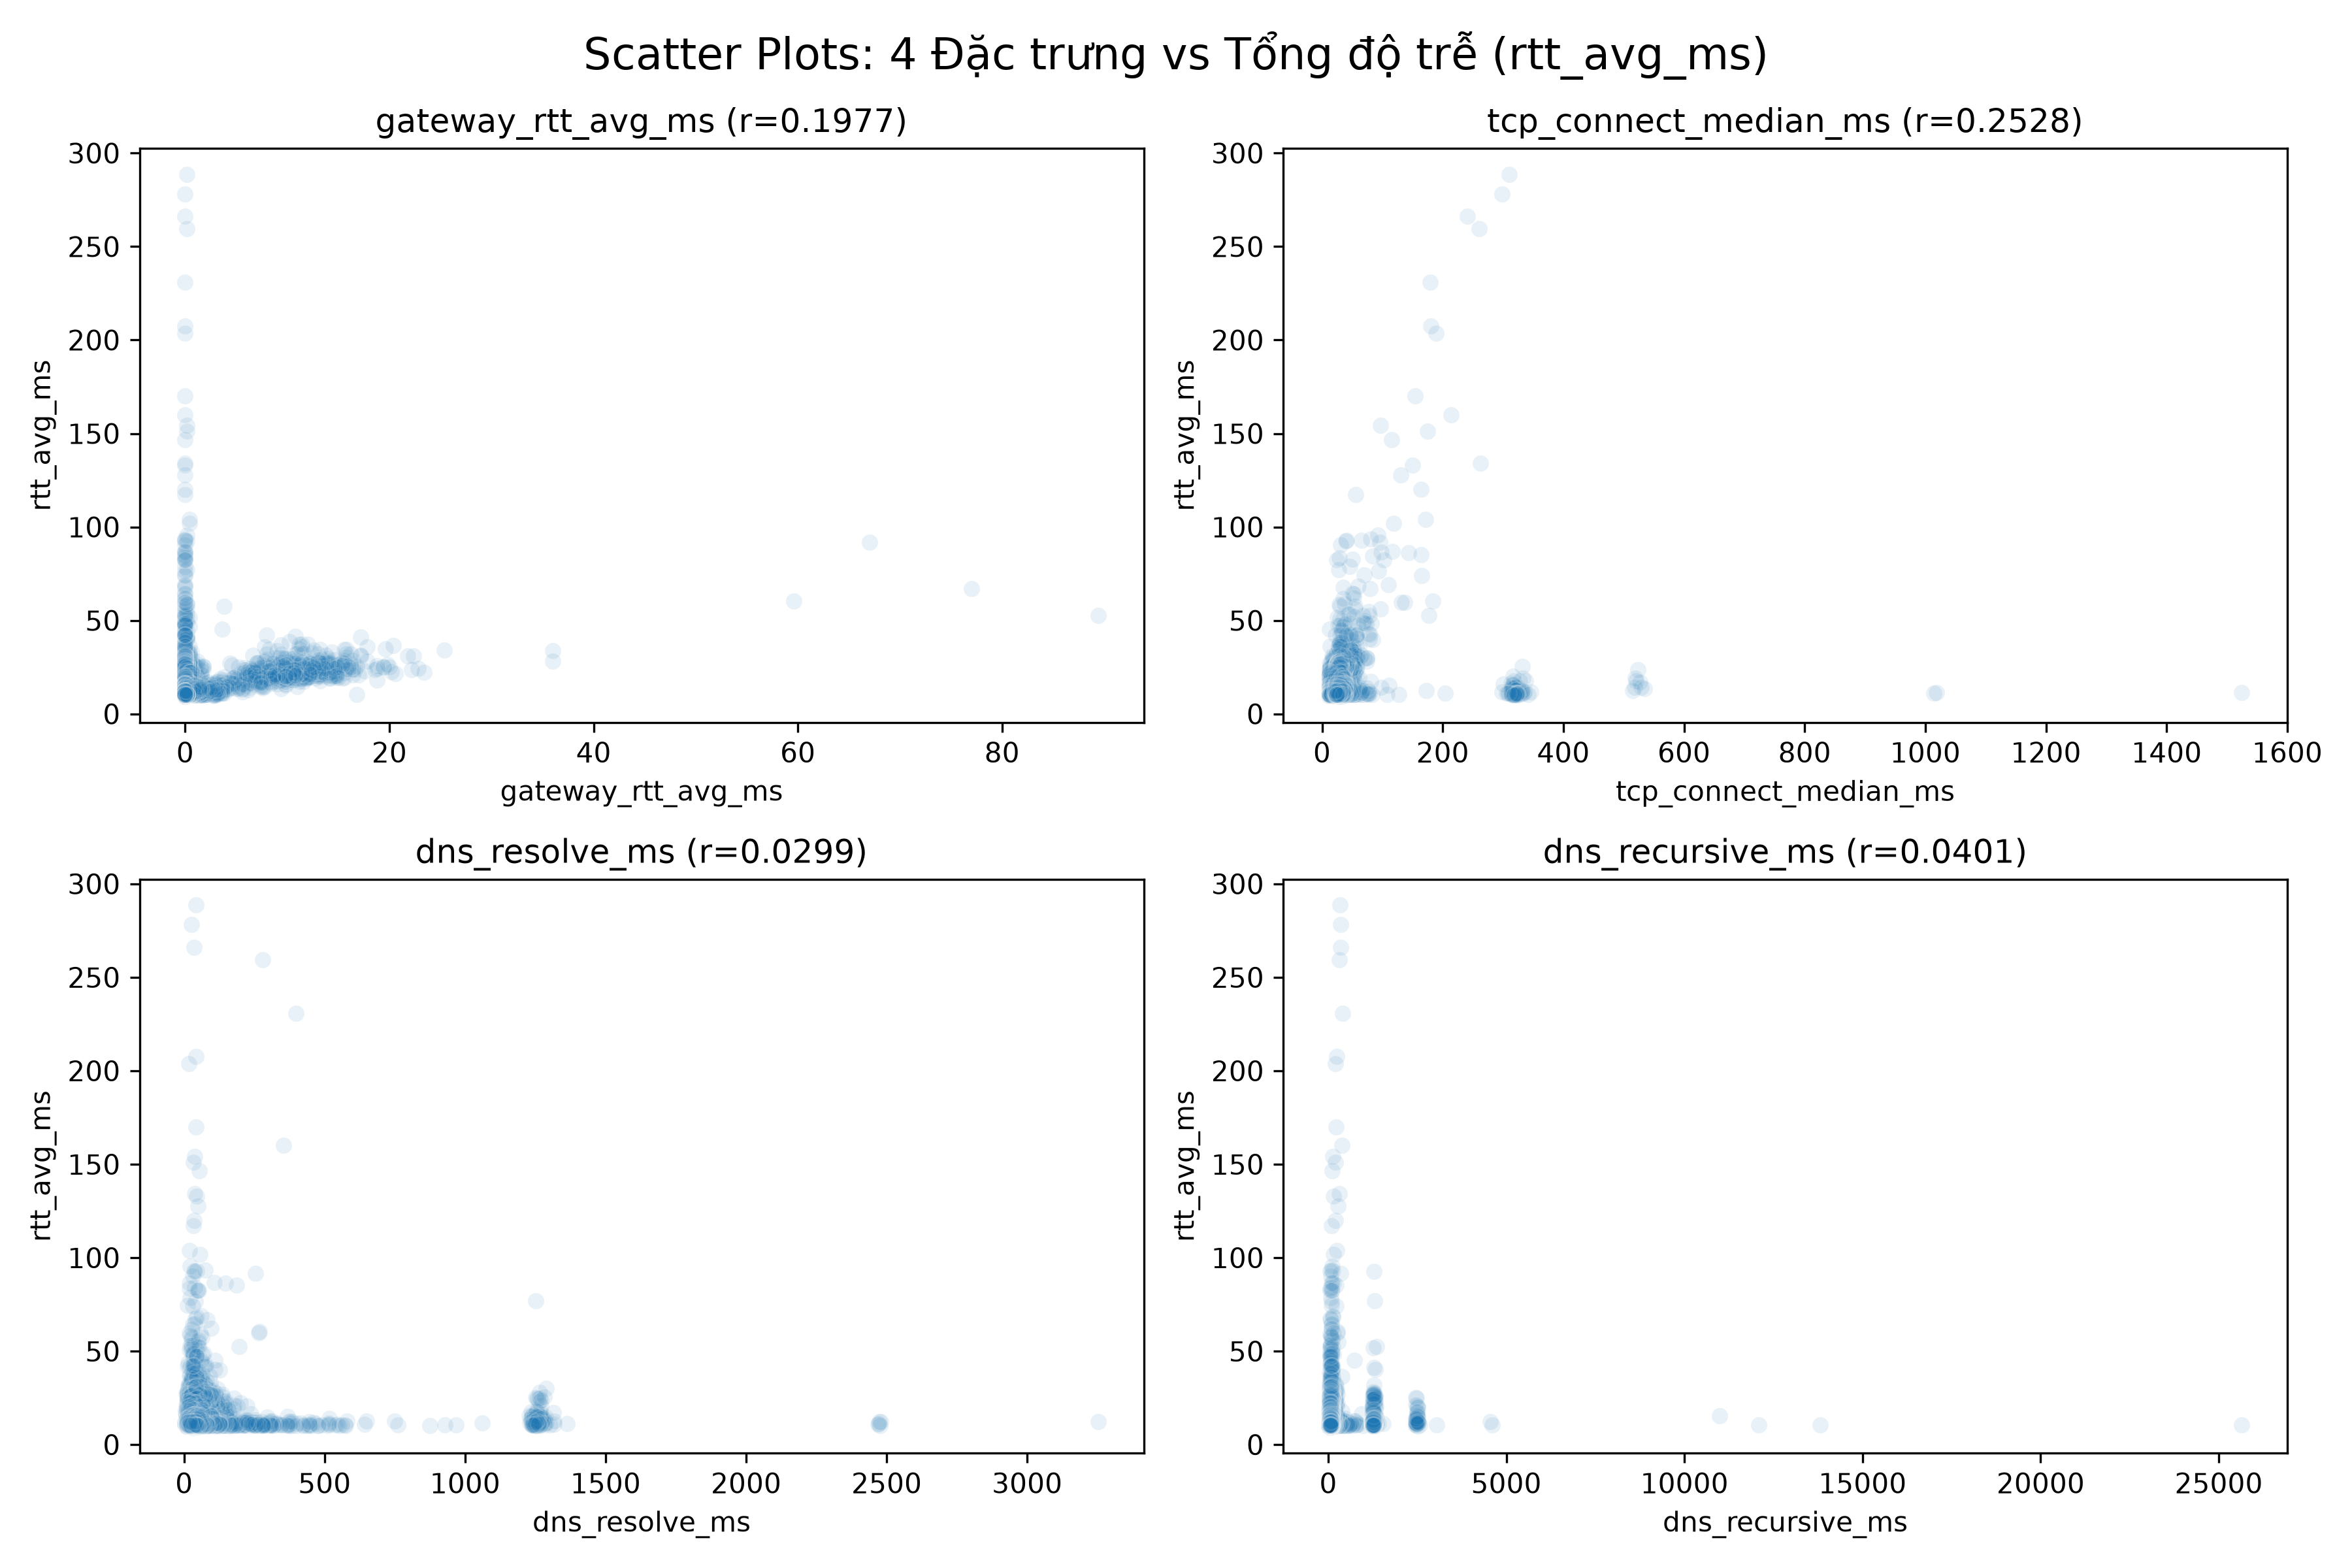
\includegraphics[width=1\textwidth]{Task2_Compare_4_Features_ScatterPlots.png}
    \caption{Biểu đồ phân tán so sánh 4 đặc trưng đầu vào với biến mục tiêu (\texttt{rtt\_avg\_ms})}
    \label{fig:scatter_4features}
\end{figure}

Từ Hình \ref{fig:scatter_4features}, ta có thể phân tích chi tiết bản chất của từng đặc trưng:
\begin{itemize}
    \item \textbf{Đặc trưng \texttt{gateway\_rtt\_avg\_ms} (Góc trên, trái):} Đồ thị thể hiện một hình chữ "L" đặc trưng. Điểm đáng chú ý nhất là có tới $25.221$ mẫu quan sát (chiếm gần một nửa tập dữ liệu) có giá trị \texttt{gateway\_rtt\_avg\_ms} bằng $0$ (Zeros = 25221). Điều này phản ánh thực tế mạng: tín hiệu gửi đến gateway (bộ định tuyến trong nhà) gần như diễn ra ngay tức khắc ($< 1$ ms). Tuy nhiên, tại chính mốc hoành độ $x=0$ này, trục tung $y$ lại phân tán dữ dội từ $10$ ms vọt thẳng lên $300$ ms. Đây chính là minh chứng trực quan cho thấy: mạng ở nhà (gateway) có thể hoàn toàn bình thường, nhưng gói tin vẫn bị trễ nghiêm trọng do nghẽn mạng quốc tế. Dạng phân bố này chắc chắn sẽ gây ra sai số lớn cho đường thẳng hồi quy tuyến tính.
    
    \item \textbf{Đặc trưng \texttt{tcp\_connect\_median\_ms} (Góc trên, phải):} Đây là biến có xu hướng tuyến tính rõ rệt nhất ($r \approx 0.2459$). Số lượng điểm Zeros bằng $0$, nghĩa là mọi kết nối TCP đều mất một khoảng thời gian nhất định để thiết lập (handshake). Các điểm dữ liệu bám theo một đường chéo dốc lên khá đồng đều, cho thấy thời gian thiết lập TCP tỷ lệ thuận khá tốt với tổng độ trễ.
    
    \item \textbf{Đặc trưng \texttt{dns\_resolve\_ms} và \texttt{dns\_recursive\_ms} (Hàng dưới):} Hai biểu đồ này thể hiện sự phân tán ngẫu nhiên, không có hình khối cụ thể. Hệ số tương quan cực kỳ thấp ($r < 0.05$) khẳng định thời gian phân giải tên miền (DNS) diễn ra độc lập và hiếm khi là nguyên nhân chính ảnh hưởng đến tổng độ trễ truyền tải của cả gói tin.
\end{itemize}
